\begin{figure} \begin{center}
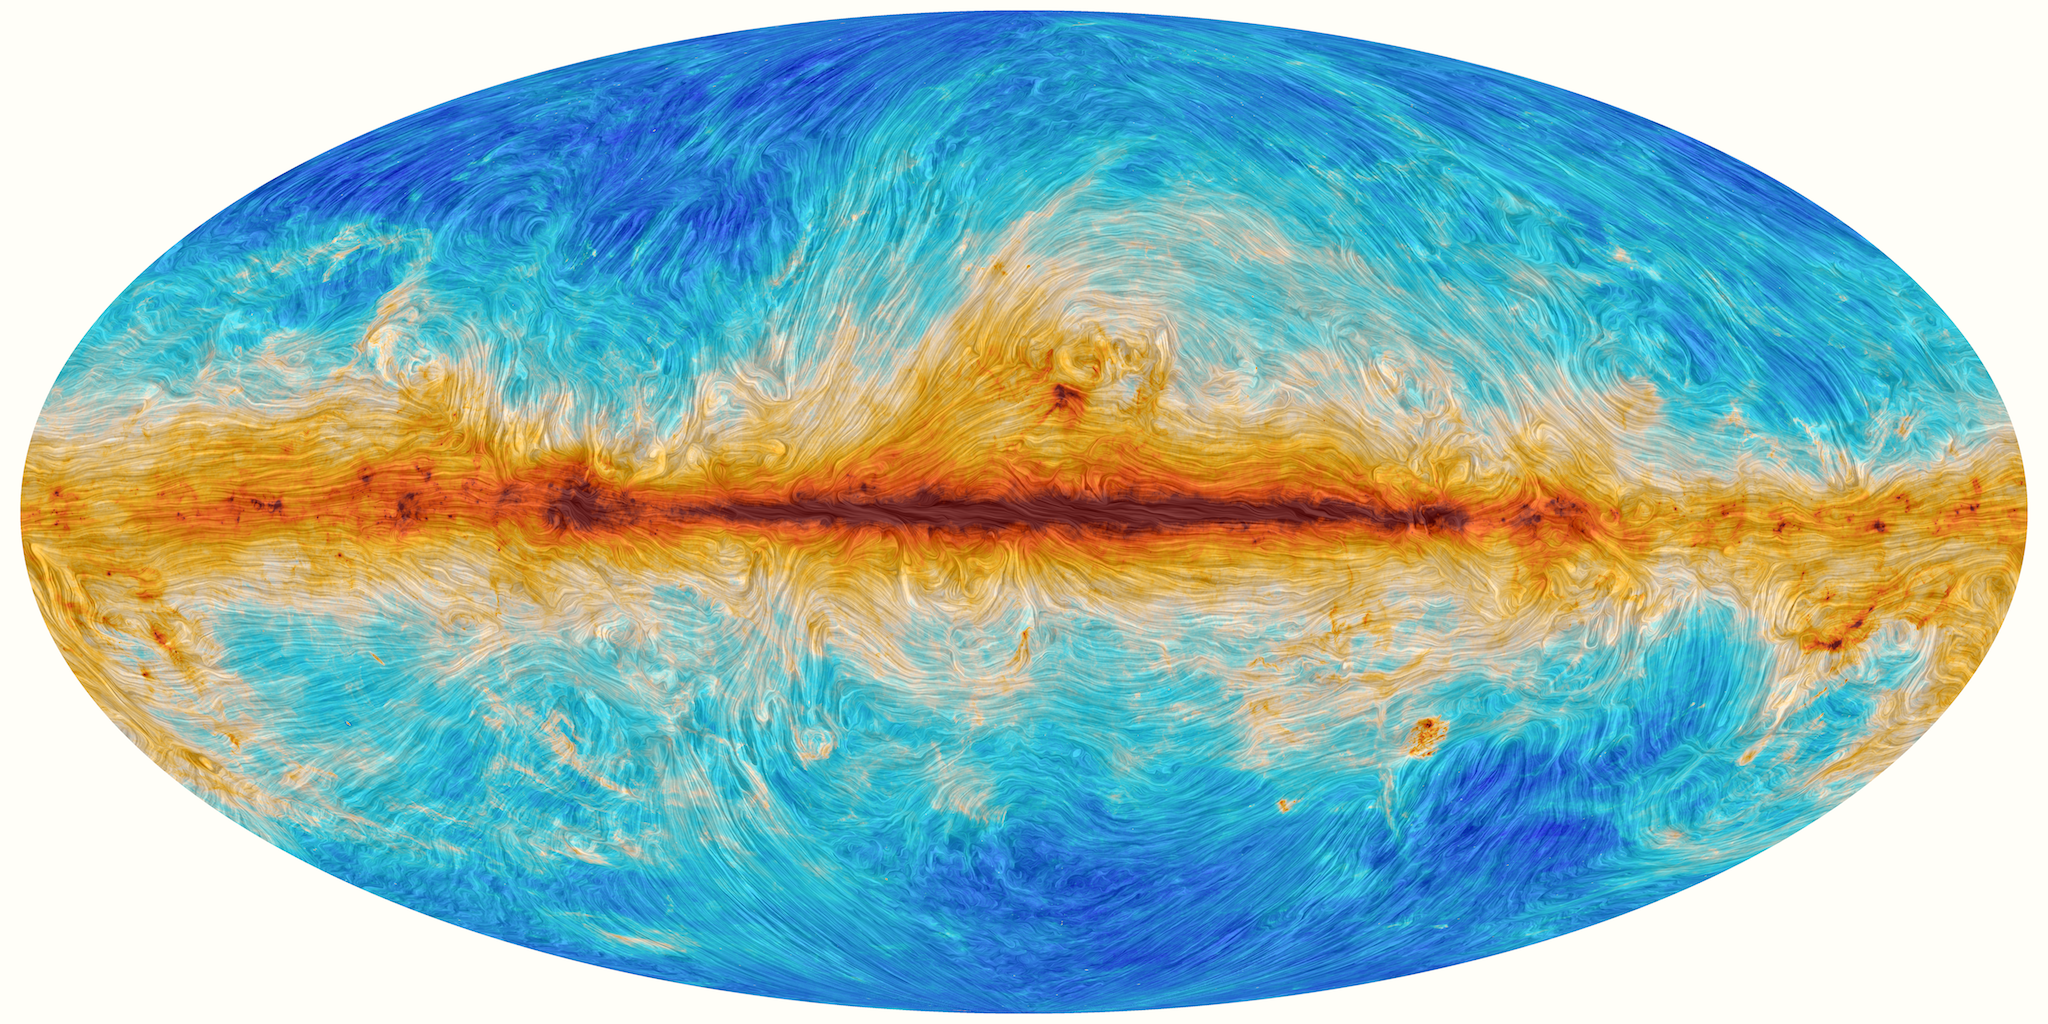
\includegraphics[width=\textwidth]{figs/2015_353GHz_B-field.png}
\caption[ ]{The large scale magnetic field of the galaxy as seen by the Planck
satellite. The color field shows dust emission at 353GHz.  The image is smeared
along the direction of the magnetic field.  \citep{PlanckXIX15}}
\label{fig.PlanckField} \end{center} \end{figure}

The \nameGalaxies\ project will simulate magnetic field generation in Milky Way
sized galaxies.  It is well know that the Milky Way has a large scale magnetic
field of roughly $\sim 6 \mu$G.  For reference, 1G is about the strength of a refrigerator
magnet.  The Galactic magnetic field can be seen in Figure \ref{fig.PlanckField}, which shows dust
emission at 353 GHz. The map is smoothed in the direction of the magnetic field,
showing large scale looping structures and small scale turbulent structures.

The origin of this magnetic field is an open question.  There are presently two
known \emph{dynamos}, that is mechanisms to amplify magnetic fields. They differ in
two ways; the length scales over which they act, and the time scales.  The fast
dynamo converts turbulent kinetic energy to magnetic energy at small scales, and
produces disordered fields quickly.  The slow dynamo produces large scale fields
slowly, with large scale convective motions. The magnetic field in the Milky Way, as well as other similar galaxies,
shows large scale order, but based on observations of galaxies, must have been
built up quickly. 

The magnetic field in the Galaxy is largely in one direction, losely following
the spiral arms.  On the way to producing a large scale magnetic field, both mechanism produce a
substantial amount of field in all directions.  Thus to have a field of mostly
one sign, the other sign must be expelled from the galaxy.  
Thus the buoyancy of the gas as
it leaves the face of the disk is important in setting the rate of growth of
the mean field.  Like many problems in physics, the answer depends sensitively
on boundary conditions, which in this case are poorly conscribed.

The circum-galactic medium (CGM) is the gas that's outside the galaxy, but still
bound to it.  It is extremely hot (millions of Kelvin) and extremely low density
(0.1 $cm^{-3}$) and thus unfortunately difficult to constrain.
The purpose of this project is to examine the growth of magnetic fields in Milky
Way sized galaxies.  
Specifically, to examine the impact of the circum-galactic
medium (CGM) properties on the dynamo. We expect that an ordered field within
the disk requires a buoyant CGM, that is gas that is expelled from the galaxy by
supernovae continues to rise, rather than falling back down immediately.  ``
